\begin{figure}[p]
    \centering
    \begin{tabular}{ll}
      \textbf{inputs:}   & \textit{B0} : pure\\
                         & \textit{cliffLeft, cliffCentre, cliffRight} : pure \\
                         & \textit{bumpLeft, bumpCenter, bumpRight} : pure \\
                         & \textit{wheelDropLeft, wheelDropRight} : pure\\
                         & acc : $\mathbb{R}^3$\\
                         & \textit{netAngle, netDistance} : $\mathbb{R}$\\
      \textbf{variables:}& \textit{driveMode} : \{FORWARD, BACKWARD, ROTATE\_LEFT, ROTATE\_RIGHT, ARC, STOP\}\\
                         & \textit{incline, tiltAngle} : $\mathbb{R}$\\
                         & \textit{turnPct} : $\mathbb{R}$\\
                         & \textit{distance, angle} : $\mathbb{R}$\\
                         & \textit{obstacleLoc} : \{LEFT, CENTRE, RIGHT\}\\
                         & \textit{offsets} : $\mathbb{R}^3$\\
                         & \textit{centreTurn} : \{\textit{true, false}\}\\
     \textbf{outputs:}   & \textit{leftWheelSpeed}, \textit{rightWheelSpeed} :  $\mathbb{R}$\\
    \end{tabular}
    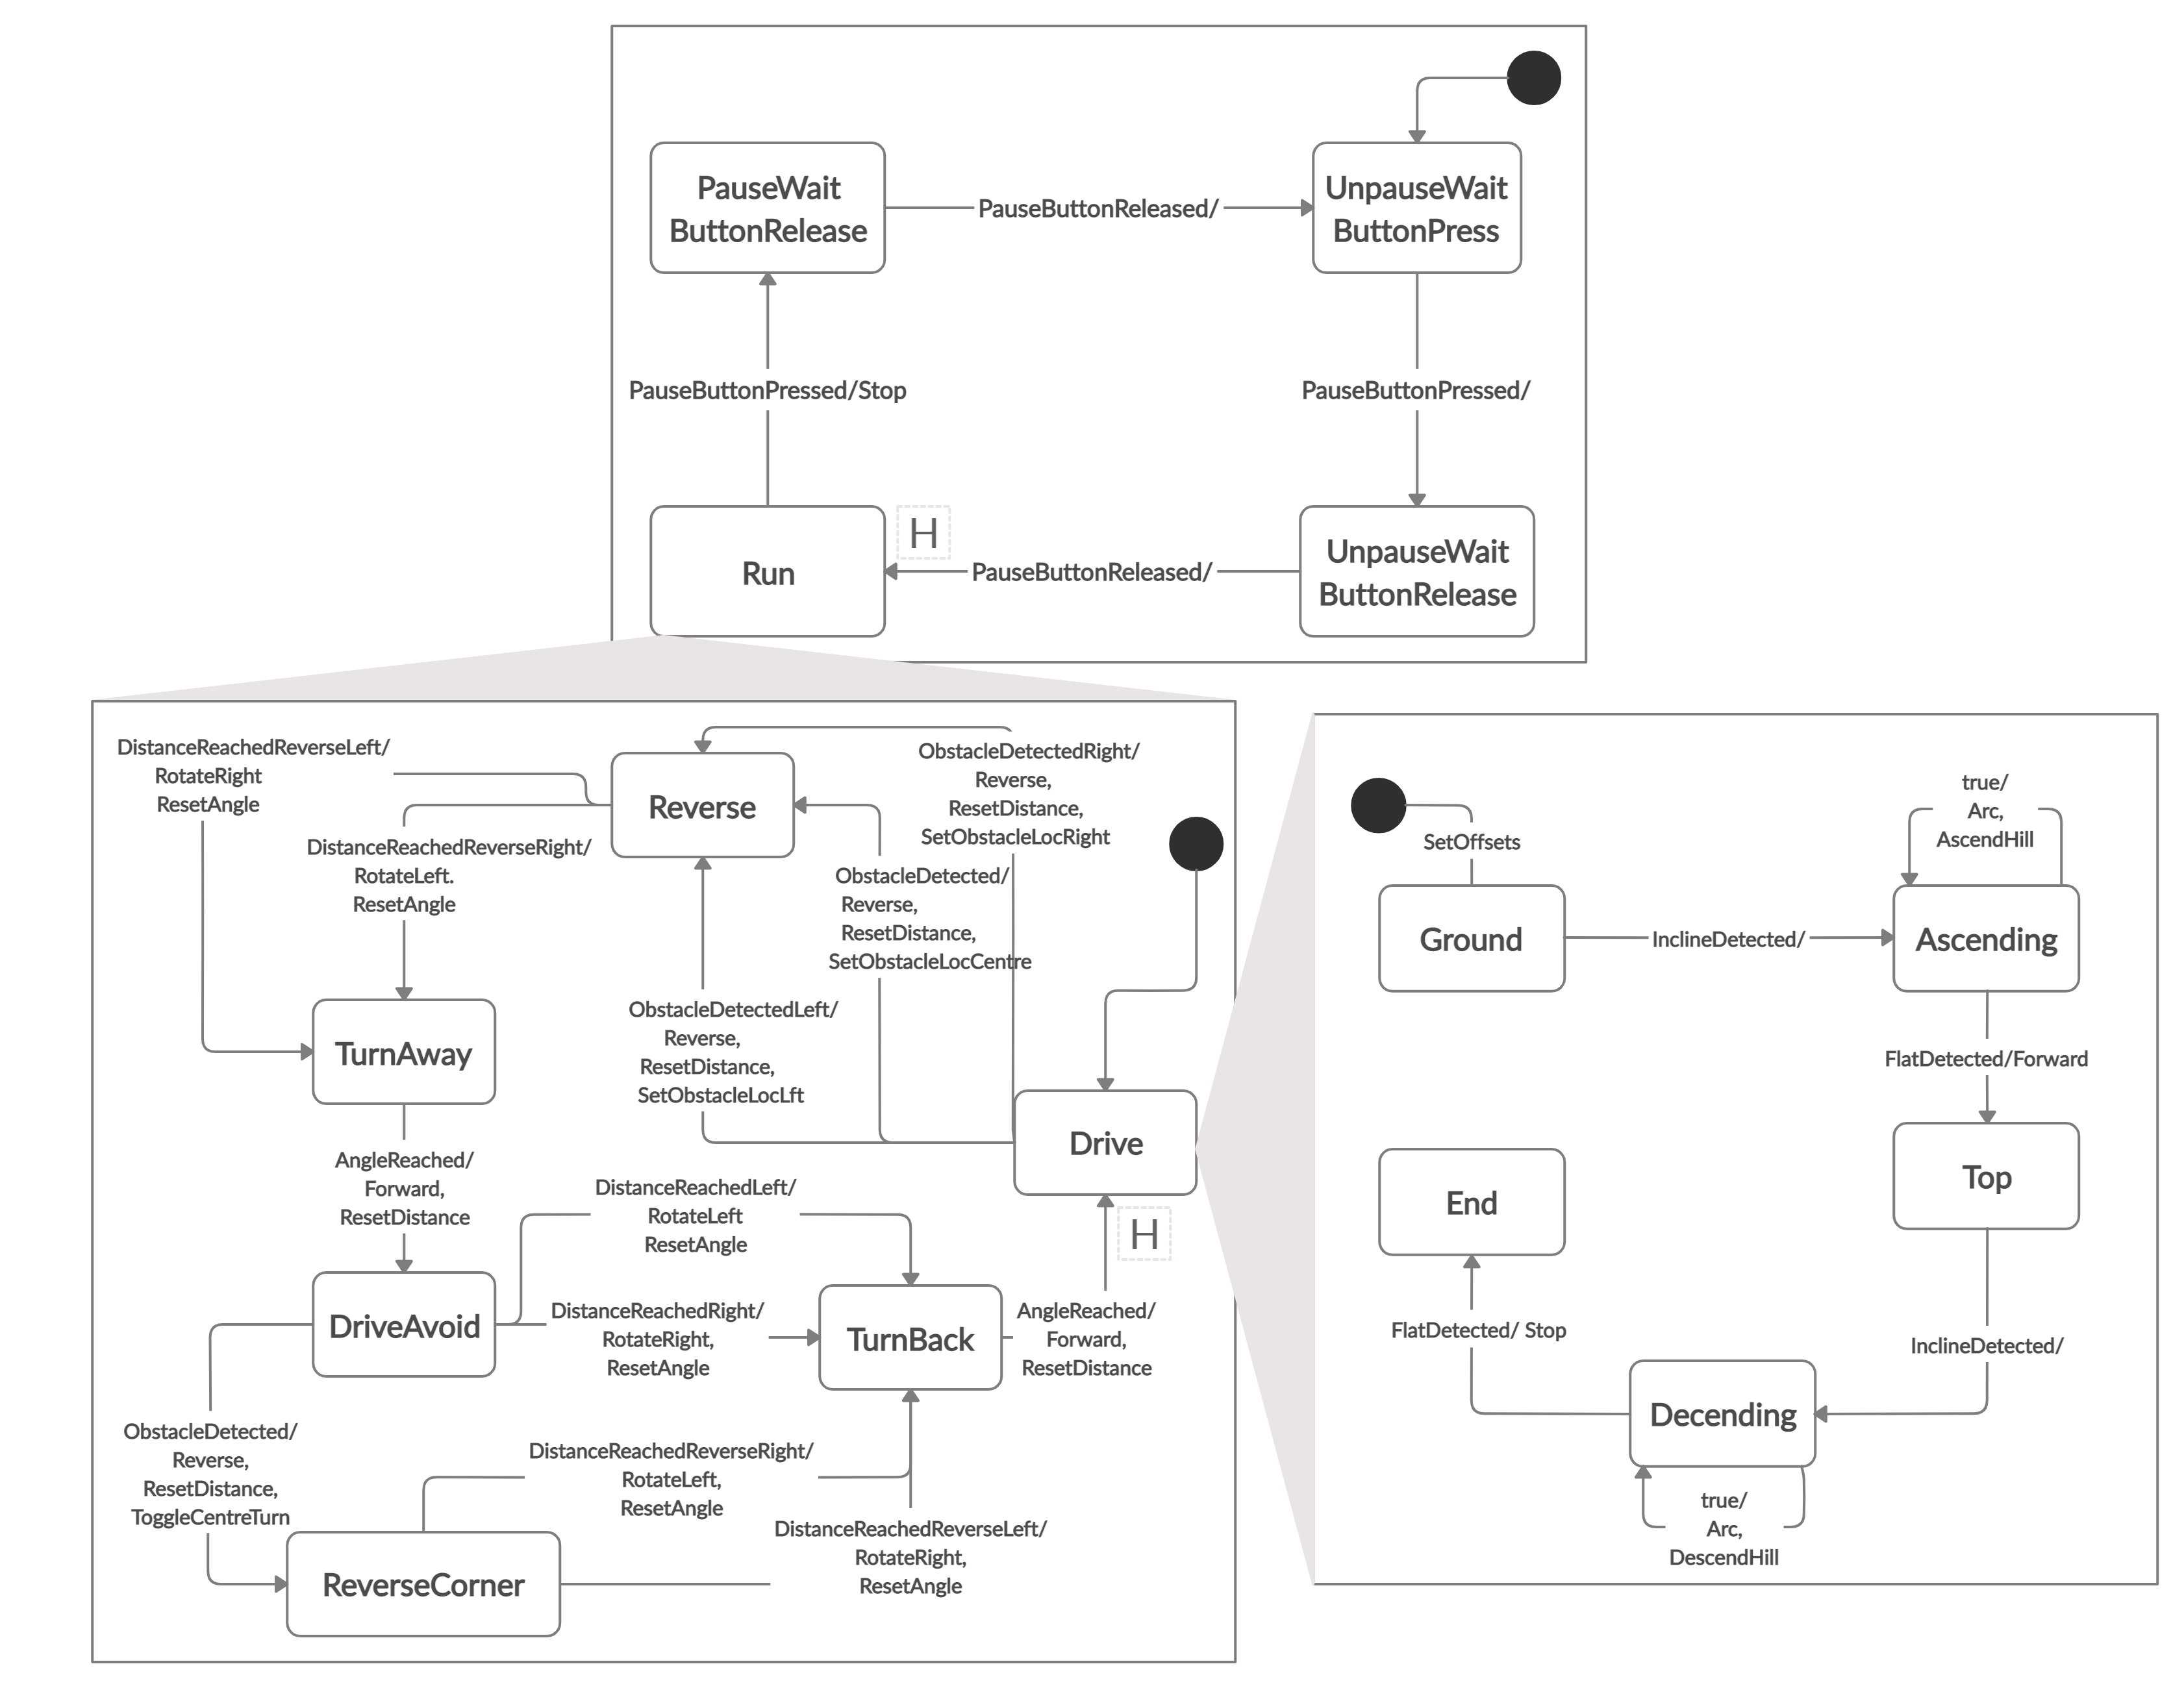
\includegraphics[width=\textwidth]{Images/Finite_State_Machine_v2.png}
    \caption{Extended State Machine (See Tables \ref{tab:triggers} and \ref{tab:actions} for Trigger and Action definitions)}
    \label{fig:FSM}
\end{figure}

\begin{table}[p]
    \centering
    \begin{tabular}{|c|c|}
        \hline
        Name        & Trigger Definition \\
        \hline\hline
        PauseButtonPressed & \textit{B0} \\
        \hline
        PauseButtonReleased    & $\neg$\textit{B0}  \\
        \hline
        ObstacleDetectedLeft & \textit{cliffLeft} $\lor$ \textit{bumpLeft} $\lor$ \textit{wheelDropLeft}\\
        \hline
        ObstacleDetectedRight & \textit{cliffRight} $\lor$ \textit{bumpRight} $\lor$ \textit{wheelDropRight}\\
        \hline
        ObstacleDetectedCentre & \textit{cliffCentre} $\lor$ \textit{bumpCentre}\\
        \hline
        ObstacleDetected & ObstacleDetectedLeft $\lor$ ObstacleDetectedRight $\lor$ ObstacleDetectedCentre\\
        \hline
        DistanceReached & abs(\textit{netDistance} - \textit{distance}) $\geq$ distanceReachedThreshold\\
        \hline
        DistanceReachedLeft & DistanceReached $\land$ (\textit{obstacleLoc} = LEFT $\lor$ \textit{centreTurn})\\
        \hline
        DistanceReachedRight & DistanceReached $\land$ $\neg$(\textit{obstacleLoc} = LEFT $\lor$ \textit{centreTurn})\\
        \hline
        DistanceReachedReverse & abs(\textit{netDistance} - \textit{distance}) $\geq$ distanceReachedReverseThreshold\\
        \hline
        DistanceReachedReverseLeft & DistanceReachedReverse $\land$ (\textit{obstacleLoc} = LEFT $\lor$ \textit{centreTurn})\\
        \hline
        DistanceReachedReverseRight & DistanceReachedReverse $\land$ $\neg$(\textit{obstacleLoc} = LEFT $\lor$ \textit{centreTurn})\\
        \hline
        AngleReached & abs(\textit{netAngle} - \textit{angle}) $\geq$ 90\\
        \hline
        FlatDetected & abs(\textit{incline)} $<$ flatDetectedThreshold\\
        \hline
        InclineDetected & abs(\textit{incline}) $>$ inclineDetectedThreshold\\
        \hline
    \end{tabular}
    \caption{Trigger Definitions}
    \label{tab:triggers}
\end{table}

\begin{table}[p]
    \centering
    \begin{tabular}{|c|c|}
        \hline
        Name        & Action Definition \\
        \hline\hline
        SetObstacleLocLeft & \textit{obstacleLoc} := LEFT \\
        \hline
        SetObstacleLocRight & \textit{obstacleLoc} := RIGHT \\
        \hline
        SetObstacleLocCentre & \textit{obstacleLoc} := CENTRE \\
        \hline
        ResetDistance & \textit{distance} := \textit{netDistance}\\
        \hline
        ResetAngle & \textit{angle} := \textit{netAngle}\\
        \hline
        Forward & \textit{driveMode} := FORWARD \\
        \hline
        Reverse & \textit{driveMode} := BACKWARD \\
        \hline
        RotateRight & \textit{driveMode} := ROTATE\_RIGHT \\
        \hline
        RotateLeft & \textit{driveMode} := ROTATE\_LEFT \\
        \hline
        Stop & \textit{driveMode} := STOP \\
        \hline
        Arc & \textit{driveMode} := ARC \\
        \hline
        AscendHill & \textit{turnPct} := $-\textit{tiltAngle}/\pi$\\
        \hline
        DescendHill & \textit{turnPct} := $-(\textit{tiltAngle}-\text{sign(\textit{tiltAngle})}\pi)/\pi$\\
        \hline
        ToggleCentreTurn & \textit{centreTurn} := $\neg$ \textit{centreTurn}\\
        \hline
        SetOffsets & \textit{offsets}:= \{\textit{acc.x}, \textit{acc.y}, $1.0-\textit{acc.z}$\}\\
        \hline
    \end{tabular}
    \caption{Action Definitions}
    \label{tab:actions}
\end{table}

\begin{table}[p]
    \centering
    \begin{tabular}{|c|c|c|}
        \hline
        \textit{DriveMode}  & \textit{leftWheelSpeed} & \textit{rightWheelSpeed} \\
        \hline\hline
        FORWARD & SPEED & SPEED \\
        \hline
        BACKWARD & $-$SPEED & $-$SPEED \\
        \hline
        ROTATE\_LEFT & $-$SPEED & SPEED \\
        \hline
        ROTATE\_RIGHT & SPEED & $-$SPEED \\
        \hline
        ARC & $\text{SPEED}(1.0-\textit{turnPct})$ & $\text{SPEED}(1.0+\textit{turnPct})$ \\
        \hline
        STOP & 0 & 0\\
        \hline
    \end{tabular}
    \caption{Output Converter}
    \label{tab:outputs}
\end{table}